\chapter{Measurements}
% \section{Voxelation, calculating distances, finding neighbors, neighbor lists, periodicity tricks\label{sec:voxelation}}
% \section{}
%
%
\section{Measuring as function of distance to matrix\label{sec:measuring_distance_to_matrix}}
\todoa{Why measure as function of distance to matrix?}
% \todoa{Finish measuring as function of distance from matrix}
% Mean distance from matrix in range --> if we limit the standard deviation as well, we're effectively limiting temperature, or diffusion??
% When measuring things like density, diffusion, and the tetrahedral order parameter in a nanoporous system, we often want to study the behaviour of 

When doing experiments with nanoporous and nanoscale systems we often want to do measures as function of the distance to the surface of the pore, in our case meaning the distance to the interface between water and silica. The first problem with this is to find out how to measure the distance from a point, for example a water molecule, to the surface. Most of our measures are done on water molecules in fractures and pores, so we first define the position of the water molecule as equal to the position of the oxygen atom in the water molecule\footnote{\hl{Something about using positions of hydrogen atoms as well as oxygen position to define water position?}}. We then use the distance from these water-oxygen atoms to the nearest silica atom to define a distance from the water molecule to the surface of the \hl{pore/fracture}. Finding the nearest silica atom isn't trivial, so a procedure for doing this is shown in \cref{sec:find_distance_to_surface}.

When measuring \hl{things} that only depend on data from one timestep we don't have to worry about that the atoms move, so we just sort the atoms by distance to the surface using the procedure in \cref{sec:find_distance_to_surface} and do our measurements, individually on each timestep. But if we want to study for example diffusion, or the tetrahedral order parameter, which depend on data from several timesteps, we have to find a good way to define which atoms are in a certain range of the surface. We tried different methods, but decided to use the average distance to the surface for this\todobo{why, examples of tested methods}.

\subsection[Note on this method]{\hl{Note on this method/distance from matrix definition}}
When we define the distance to the silica matrix as the distance to the nearest silicon atom, we get some effects we should take note of for atoms very close to the matrix. With our definition of the distance to the silica matrix we are effectively making our bins out of spherical shells centered on each silicon atom. Compared to for example using the $z$-distance to the surface in a completely flat fracture, where we know the $z$-height of the surface, we see that this can give different results. The problem is of course that in a random fracture in a silica system we can't easily define a normal vector to the surface of the fracture, so finding an equivalent to the $z$-distance in such a fracture is hard.

When we do our measurements as a function of distance to the silica matrix we usually sort the atoms into bins according to their \hl{(average)} distance to the nearest silicon atom. At distances much larger than the average distance between the silicon atoms at the surface of the fracture this isn't a problem, since the curature of the spherical shells is low, and the volume enclosed by the shells is pretty close to the one we would have gotten if we had created bins used $z$-positions in flat fracture. But at distances close to the average distances between the silicon atoms we begin to see that the volumes our bins consist of start curving around the silicon atoms, instead of staying flat as they would have if we were using the $z$-distance. See \cref{fig:distance_to_matrix_illustration} for an illustration of this. In this illustration we have illustrated bins created using the same bin width and distance from the matrix, using the two different methods. The dark gray areas are the ones that are included using both methods ($A_\text{Si}\cap A_z$), the light grey areas ($A_\text{Si}$) are the ones unique to the spherical shell bins, and the yellow areas are the ones unique to the the $z$-distance bins ($A_z$).%
%
\begin{figure}[htpb]%
% \centering%
    \begin{minipage}[c]{0.6\textwidth}%
        \captionsetup{width=0.925\textwidth}%
        \centering%
        \includesvg[width=\textwidth, svgpath=./images/density/]{number_of_molecules_all_distances02}%
        \caption{%
            Plot of the number of atoms in each bin when measuring \hl{something} as a function of distance to the \hl{silica matrix/surface of the fracture}. \hl{Finish caption}%
            \label{fig:distance_to_matrix_number_of_atoms}%
        }%
    \end{minipage}%
    \hfill%
    \begin{minipage}[c]{0.3999\textwidth}% % change "b" to "t" to anchor top instead of bottom
%         \captionsetup{width=0.95\textwidth}% % minipage defines a \textwidth for it's own, so we have to repeat this command inside the minipage
        \captionsetup{width=0.9\textwidth}% % minipage defines a \textwidth for it's own, so we have to repeat this command inside the minipage
        \centering%
        \includesvg[pretex=\normalsize, width=0.9\textwidth, svgpath=./images/distance_to_matrix_illustration/]{figure12}%
        \caption{%
            Illustration of binning when using distance to nearest silicon atom as definition of distance to silica matrix ($r_\text{Si})$, vs. $z$-distance ($r_z$). \hl{Finish caption}%
            \label{fig:distance_to_matrix_illustration}%
        }%
    \end{minipage}%
\end{figure}%

This difference in binning is something we should be wary about when comparing our results to measurements done using the $z$-distance as the distance to the matrix. One result of this can be seen in \cref{fig:distance_to_matrix_number_of_atoms}, where we have plotted the number of atoms in each bin of width $0.25\text{ \AA}$ against the distance from the silica matrix (meaning the radius of the spherical shells). We see that we get no atoms in the bins from 2 to 3 \Ang, but a big spike just below 2 \AA. This spike is most likely caused by water-oxygen atoms that are bound to silicon atoms, which we placed there when passivating the system (silicon-water atoms from the initial silica crystal are not included in the counting, but we use water-oxygen when passivating). If we would have used the $z$-distance in a flat fracture in a system like this, we would most likely have gotten a very different distribution below 4 \AA\todobo{Why?}, with a more flat distribution instead of it going to zero, since the angular distribution of the oxygen atoms around the silica atoms \hl{makes the $z$-distance vary}.
% \begin{figure}[htpb]%
%     \centering%
%     \includesvg[width=0.8\textwidth, svgpath=./images/density/]{number_of_molecules_all_distances01}%
%     \caption{%
%         Number of atoms in each bin when measuring density of water as function of distance from matrix. Bin width = 0.25 \AA\ \hl{FINISH CAPTION}. %
% %         \label{fig:cell_lists}%
%     }%
% \end{figure}%
% %
% \begin{figure}[htpb]%
%     \centering%
%     \includesvg[width=0.4\textwidth, svgpath=./images/distance_to_matrix_illustration/]{figure05}%
%     \caption{%
%         \hl{CAPTION}. %
% %         \label{fig:cell_lists}%
%     }%
% \end{figure}%
%
%
% %
% \begin{figure}[htpb]%
%     \centering%
%     \setlength{\myfigwidth}{0.49\textwidth}%
% %     \setlength{\mycaptionwidth}{0.3\textwidth}%
% %
%     \begin{subfigure}[b]{\myfigwidth}%
%         \centering% % Need to center to get image centered over caption
%         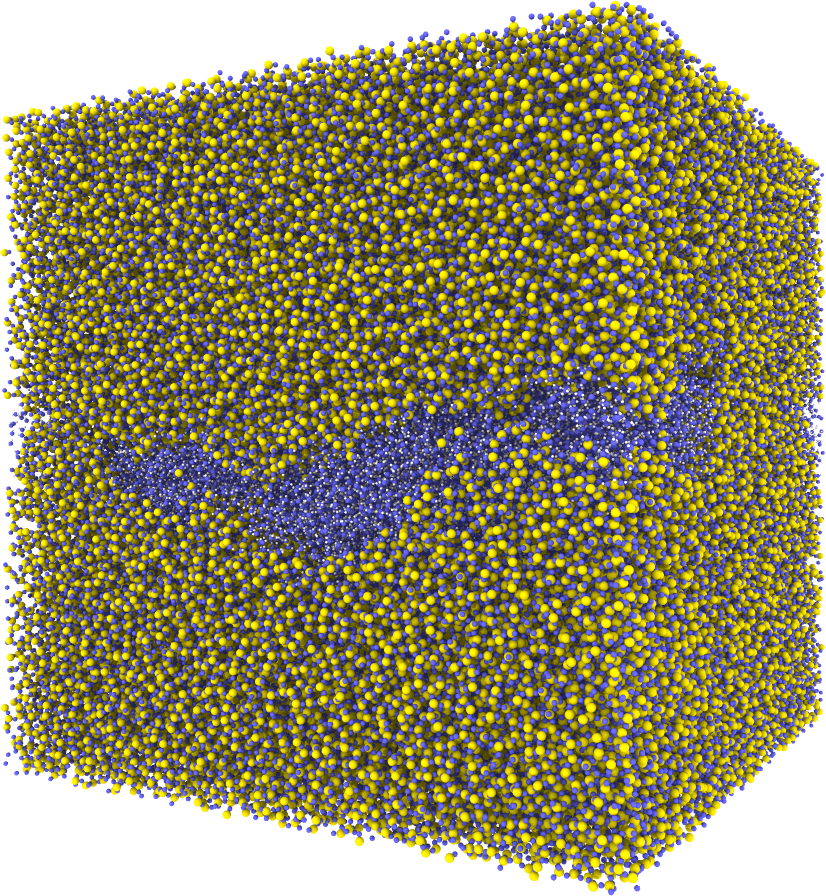
\includegraphics[width=\textwidth]{images/systems/trimmed-rough_fracture01_abel_13}%
%         \caption{Caption.}%
% %         \label{fig:hex_to_tetra}%
%     \end{subfigure}%
%     \hfill%
%         \begin{subfigure}[b]{\myfigwidth}%
%         \centering% % Need to center to get image centered over caption
%         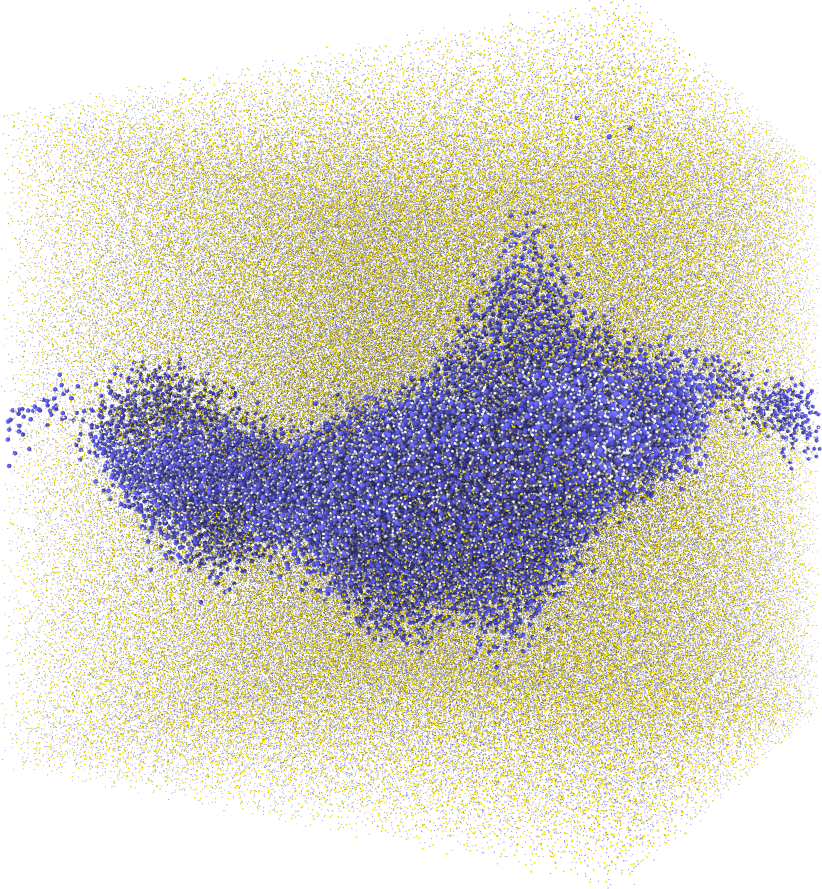
\includegraphics[width=\textwidth]{images/systems/trimmed-rough_fracture01_abel_15}%
%         \caption{Caption.}%
% %         \label{fig:hex_to_tetra}%
%     \end{subfigure}%
%     \\%
%     \begin{subfigure}[b]{\myfigwidth}%
%         \centering% % Need to center to get image centered over caption
%         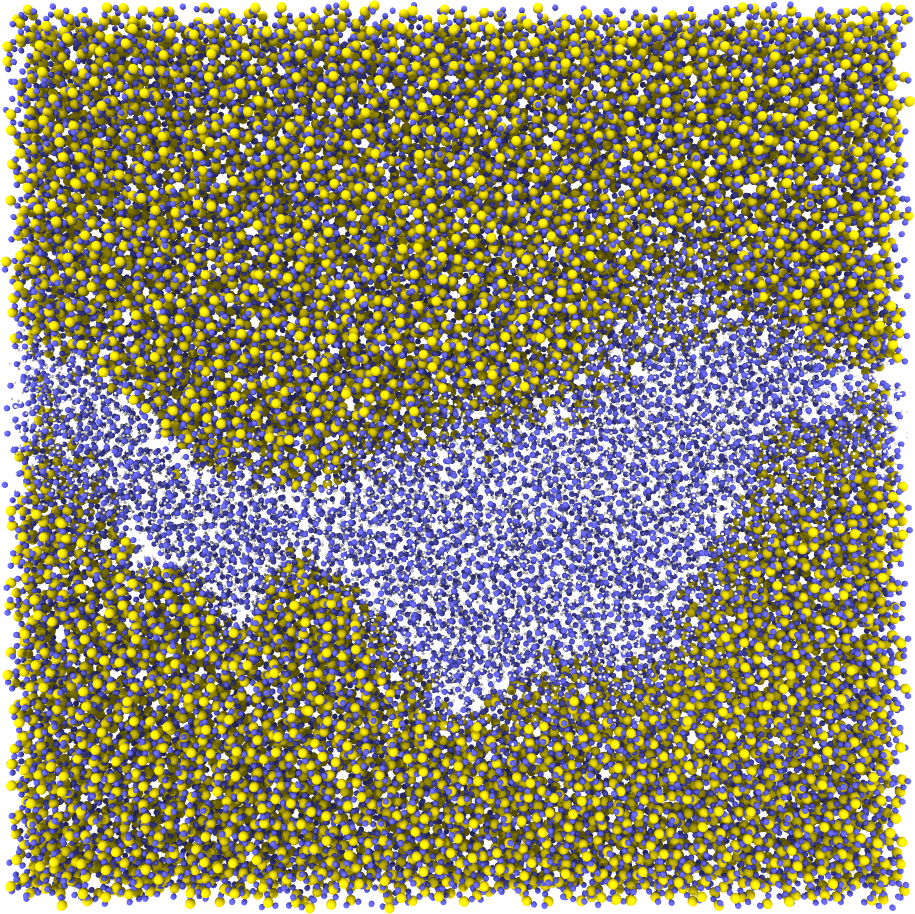
\includegraphics[width=\textwidth]{images/systems/trimmed-rough_fracture01_abel_16}%
%         \caption{Caption.}%
% %         \label{fig:hex_to_tetra}%
%     \end{subfigure}%
%     \hfill%
%     \begin{subfigure}[b]{\myfigwidth}%
%         \centering% % Need to center to get image centered over caption
%         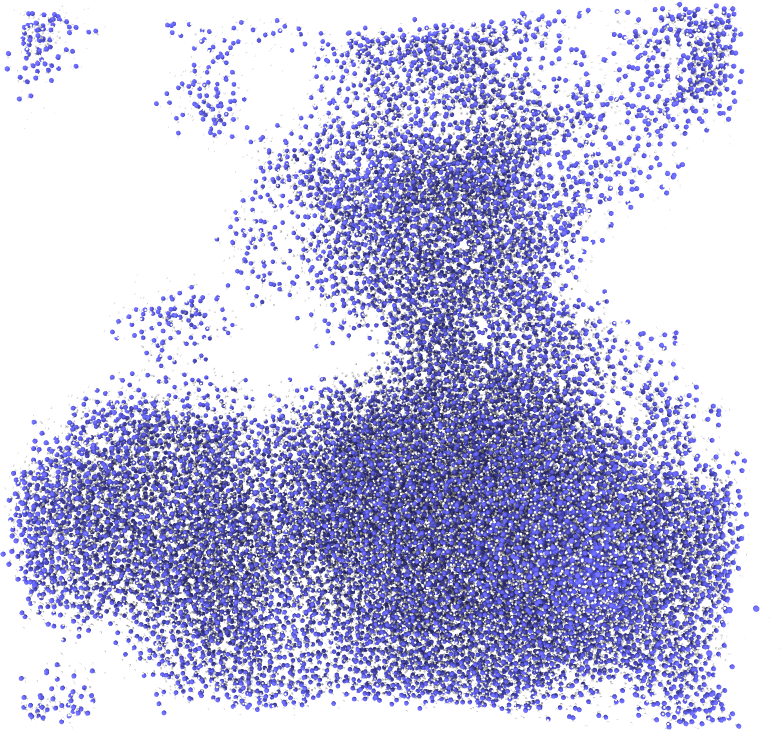
\includegraphics[width=\textwidth]{images/systems/trimmed-rough_fracture01_abel_17}%
%         \caption{Caption.}%
% %         \label{fig:hex_to_tetra}%
%     \end{subfigure}%
%     \caption{%
%         Caption. %
%         \label{fig:rough_fracture01}%
%     }%
% \end{figure}%

\section{Voxelation\label{sec:voxelation}}
The method of voxelation is a method where we divide our simulation system into adjacent boxes or \emph{voxels} (3-dimensional pixels). The system is divided into $n_x\times n_y\times n_z$ voxels of size $l_x\times l_y\times l_z$. Depending the what we want to calculate we can calculate the voxel size from the number of voxels, or vice versa, using the following relation
\begin{align*}
    n_i = \frac{L_i}{l_i},
\end{align*}
where $L_i$ is the system size, and we assume that the voxel size $l_i$ is set so that $L_i$ is evenly divisible by $l_i$\hl{, meaning that the remainder of $L_i/l_i$ is zero}. If we have a maximum or minimum voxel size $l_i^\text{max}$ or $l_i^\text{min}$ we can use the following relations to calculate the number of voxels
\begin{align*}
    &n_i=\left\lfloor\frac{L_i}{l_i^\text{max}}\right\rfloor &\text{or}& &n_i=\left\lceil\frac{L_i}{l_i^\text{min}}\right\rceil,
\end{align*}
where $\lfloor x \rfloor$ is the \Verb!floor!-function and $\lceil x \rceil$ is the \Verb!ceil!-function.

The voxels are indexed $(i,j,k)$ where $i,j,k \in [0,n_i-1]$, and a voxel is defined as the points $(x,y,z)$ where
\begin{align}
    \left\lfloor\frac{x}{l_x}\right\rfloor = i,\label{eq:find_voxel_index}
\end{align}
and similarly for the other dimensions.

\subsection{Neighbor lists\label{sec:neighbor_lists}}
When doing calculations and measurements on a molecular system, we often need information about the neighboring atoms of each atom, and we want to make a so-called \emph{neighbor list}, which are lists of which atoms are within a distance $dr$ of each atom. Finding out which atoms are within a certain distance of each atom can take a long time; the trivial way of checking each atom against all other atoms scales as $\mathcal{O}(N^2)$, $N$ being the number of atoms. 
%
%There are many clever algorithms for finding nearest neighbors, often called a ``nearest neighbor search'' (see \url{http://www.slac.stanford.edu/cgi-wrap/getdoc/slac-r-186.pdf} and references in that paper, especially ``11. Levinthal 1966''). 

Since we want to find all neighbors within a distance $dr$ of a point, for all or most of the atoms, we can use the voxelation method to do it efficiently. To do this we first voxelate the system using a minimum voxel size equal to $r$. We then find which voxel each atom belongs to, and store this. We can then find the atoms within a distance $dr$ from a point $(x,y,z)$ by first finding the voxel this point lies in using (from \cref{eq:find_voxel_index})
\begin{align*}
    &i = \Bigg\lfloor \frac{x}{l_x} \Bigg\rfloor,& &j = \Bigg\lfloor \frac{y}{l_y} \Bigg\rfloor,& &j = \Bigg\lfloor \frac{z}{l_z} \Bigg\rfloor,&
\end{align*}
where $l_x\times l_y \times l_z$ is the actual voxel size (we need an even number of voxels, so the actual voxel size is governed by the system size). We then check the distance between the point and the atoms in the voxel the point belongs in, and the atoms in the 26 neighboring voxels of this voxel. 
\todoc{make voxel size vs. $dr$ illustration}%

Checking the 26 neighboring voxels ensure that we included all atoms within the distance $dr$. We can see this by looking at the worst case example, where we have a point right at the edge of the voxel it belongs to, at $(i+(1-\epsilon_0))$, and an atom in voxel $(i+2)$ being as close to the point as possible, at $(i+2 + \epsilon)$. The distance between those two points would then be
\begin{align*}
    ((i+2)l + \epsilon_1) - (il + (l-\epsilon_0)) 
    &= ((i + 2) - (i + 1) - \epsilon_0)l + \epsilon_1 + \epsilon_0 \\
    &= l + \epsilon + \epsilon_0,
\end{align*}
which is larger than $l$, since $\epsilon_0, \epsilon_1$ have to be larger than 0.

When voxelating the system using the distance $r$ we should take care not to use a too small distance, i.e. make the voxels too small and create a lot of voxels. Since the total number of voxels goes as $n^3$ the memory needed to store the matrix increases rapidly with decreasing voxel size. To avoid this we usually implement a hard limit to the number of voxels, and found that a limit of $n < 256$ or even $n < 128$ seemed to work good in most cases. On the other hand, if we make the voxels too large we soon find that the program isn't especially efficient. This is because most voxels will have a lot of atoms in then, and we have to look through a lot of atoms when checking the 26+1 voxels for each atom.

An implementation of the voxelation method for creating neighbor lists can be seen in \cref{list:create_neighbor_lists}. Note that when calculating distances between points we usually calculate and compare squared distances like $r^2 = (x_1-x_2)(x_1-x_2) + \dots$, since calculating roots are a time-consuming operation on a computer (at least compared to multiplication and addition).
%
% We didn't find any algorithms for solving this specific problem, and the usual algorithms can't benefit from the fact that we need to find the nearest neighbors of \emph{all} points.
%
\begin{listing}[!htb]%
\begin{cppcode*}{gobble=4}
    int nVoxels = floor(systemSize/radius);
    double voxelSize = systemSize*nVoxels;
    
    sortAtomsIntoVoxels(atoms, voxelSize, voxels);
    
    vector<vector<Atom*> > neighborAtoms(atoms.size());
    
    // Loop over all atoms
    for (Atom *atom : atoms) {
        // Index of the voxel this atom belongs to
        ivec3 index = floor(atom.position() / voxelSize)
        
        // Loop over all 27 neighbor voxels (including self)
        for (int di = -1; di <= 1; di++)
        for (int dj = -1; dj <= 1; dj++)
        for (int dk = -1; dk <= 1; dk++)
        {{{
            // Index of neighbor voxel using periodic boundary conditions
            // nx, ny, nz is the number of voxels in each direction
            int i = (index[0] + di + nx) % nx;
            int j = (index[1] + dj + ny) % ny;
            int k = (index[2] + dk + nz) % nz;
            
            neighborAtoms[atom.index()].push_back(
                findAtomsWithinRadius(atom, voxels[i][j][k], radiusSquared)
            );
        }}}
    }
\end{cppcode*}
\caption{%
    An example of how to find the neighbor atoms within a given distance (\mono{radius}) of all atoms. This example assumes a cubic system of size \mono{systemSize}. See \cref{list:sortAtomsIntoVoxels,list:findAtomsWithinRadius} for example implentations of \mono{sortAtomsIntoVoxels} and \mono{findAtomsWithinRadius}. %
    \label{list:create_neighbor_lists}%
}%
\end{listing}%
%
\begin{listing}[!htb]%
\begin{cppcode*}{gobble=4}
    void sortAtomsIntoVoxels(
        const vector<Atom*> &atoms, 
        double voxelSize, 
        vector<vector<vector<Atom*> > > &voxels) {
        
        for (Atom *atom : atoms) {
            // Index of the voxel this atom belongs to
            int i = floor(atom.position().x() / voxelSize);
            int j = floor(atom.position().y() / voxelSize);
            int k = floor(atom.position().z() / voxelSize);
            voxels[i][j][k].push_back(atom);
        }
    }
\end{cppcode*}
\caption{%
    Example of implementation of \mono{sortAtomsIntoVoxels} from \cref{list:create_neighbor_lists}, for sorting atoms into voxels with size \mono{voxelSize}. We use the \mono{floor} function to get the index of the voxel each atom belongs in, using zero-based numbering. % \mono{sortAtomsIntoVoxels}. %
    \label{list:sortAtomsIntoVoxels}%
}%
\end{listing}%
\begin{listing}[!htb]%
\begin{cppcode*}{gobble=4}
    vector<Atom*> findAtomsWithinRadius(
        Atom *atom1, const vector<Atom*> &voxel, double radiusSquared) {
        
        vector<Atom*> neighborAtoms;
        
        // Loop over atoms in neighbor voxel
        for (Atom *atom2 : voxel) {
            if (atom2 != atom1) {
                double drSquared = 
                    calculateDistanceSquaredBetweenAtoms(atom1, atom2);
                if (drSquared < radiusSquared) {
                    neighborAtoms.push_back(atom2);
                }
            }
        }
        return neighborAtoms;
    }
\end{cppcode*}
\caption{%
    Example implementation of \mono{findAtomsWithinRadius} from \cref{list:create_neighbor_lists}. See \cref{list:calculateDistanceSquaredBetweenAtoms} for an example implementation of \mono{calculateDistanceSquaredBetweenAtoms}.%
    \label{list:findAtomsWithinRadius}%
}%
\end{listing}%
%
\begin{listing}[!htb]%
\begin{cppcode*}{gobble=4}
    double calculateDistanceSquaredBetweenAtoms(Atom *atom1, Atom *atom2) {
        vec3 dr = atom2->position() - atom1->position();
        
        // Minimum image convention
        for (int dim = 0; dim < 3; dim++) {
            if      (dr[dim] >  L[dim]/2.0) dr[dim] -= L[dim];
            else if (dr[dim] < -L[dim]/2.0) dr[dim] += L[dim];
        }
        
        // Calculate $dr^2$ instead of $\sqrt{dr^2}$, since sqrt() is a very 
        // slow operation, and in this case is unnecessary
        return dr.lengthSquared();
    }
\end{cppcode*}
\caption{%
    Example implementation of \mono{calculateDistanceSquaredBetweenAtoms} from \cref{list:findAtomsWithinRadius}.%
    \label{list:calculateDistanceSquaredBetweenAtoms}%
}%
\end{listing}%

\subsection{Finding distance to surface\label{sec:find_distance_to_surface}}
When doing measurements on water molecules we often want to know the distance from the water molecule to the surface of the pore the water molecule is in. To find this we first define the position of the water molecule as the position of the oxygen atom in the molecule. We then use the distance between this oxygen atom to the nearest silicon atom as the distance to the surface.

To use the voxelation method we need to have a maximum distance to look for silicon atoms in. This atom should be set as small as possible, to efficiently use the voxelation method\footnote{We usually implement a hard upper bound on the number of voxels, or a lower bound on the voxel size, to keep the memory consumption of our program in check}. We divide the system into voxels using the technique from \cref{sec:voxelation}, and sort all silicon atoms into the voxels. For each water-oxygen atom we then find the distance to the nearest silicon atom by calculating the distance between the oxygen atom and the silicon atoms in the voxel the oxygen atom belongs in, and the silicon atoms in all 26 neighbor voxels. See \cref{sec:neighbor_lists} for more details.

\FloatBarrier
\section{Density}
To measure the density in a uniform system consisting of just one atom type, we can use
\[
    \rho = \frac{Nm}{V},
\]
where $N$ is the number of atoms, $m$ the mass of an atom, and $V$ the volume of the whole system. But if we have a more complicated system, like in our case where we have three different atom types, liquid water in some parts of the system, and solid silica in other parts, we can't use that simple relation. What we do instead is to assiociate a volume $V_i^j$ with each atom of type $j$, and calculate the density of atom type $j$ using
\[
    \rho_j = \dfrac{m_jM}{\sum_{i=0}^M V_i^j},
\]
where $m_j$ is the mass an atom of type $j$, and $M$ is the number of atoms of type $j$. \hl{We identify as the $\rho_j/m_j$ number density.} We can find the mass of an atom type from standard tables of molar masses, but we still need to find the volumes $V_i^j$ associated with each atom. To do this we use something called \hl{Voronoi cells/Voronoi tesselation}\todobo{citation? Dirchlet 1850 and Voronoi 1908, so very old...}. Voronoi tesselation is done by dividing the system into non-overlapping convex polyhedra (or convex polygons in 2 dimensions), with one atom in each polyhedra. The volume inside the polyhedron surrounding each atom consists of all points in space closer to that atom than any other atom. 

We use the \cpp-library \texttt{Voro++} to find the Voronoi cells, and calculate the volumes of the cells. See \cref{fig:2d_voronoi_diagram} for an illustration of a 2-dimensional Voronoi, and \cref{fig:3d_voronoi_diagram} for a rendering of a 3D Voronoi diagram.
%
\begin{figure}[htpb]%
% \centering%
    \begin{minipage}[t]{0.485\textwidth}%
        \captionsetup{width=\textwidth}%
        \centering%
%         \includesvg[width=0.8\textwidth, svgpath=./images/voronoi/]{2d_diagram03}%
        \includesvg[height=0.7\textwidth, svgpath=./images/voronoi/]{2d_diagram06_overlapping}%
        \caption{%
            Illustration of Voronoi cells in 2 dimensions. Freely after Wikipedia Commons\cite{wikiVoronoiImage}.%
            \label{fig:2d_voronoi_diagram}%
        }%
    \end{minipage}%
    \hfill%
    \begin{minipage}[t]{0.485\textwidth}% % change "b" to "t" to anchor top instead of bottom
    \captionsetup{width=\textwidth}% % minipage defines a \textwidth for it's own, so we have to repeat this command inside the minipage
        \centering%
%         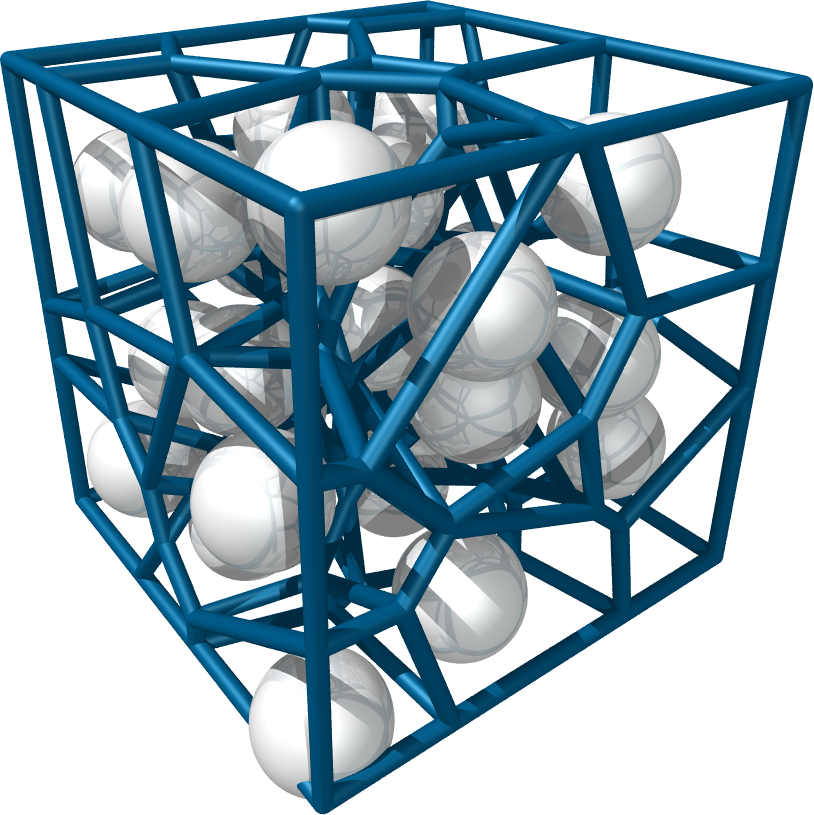
\includegraphics[width=0.8\textwidth]{images/voronoi/3d_diagram04_crop.png}%
        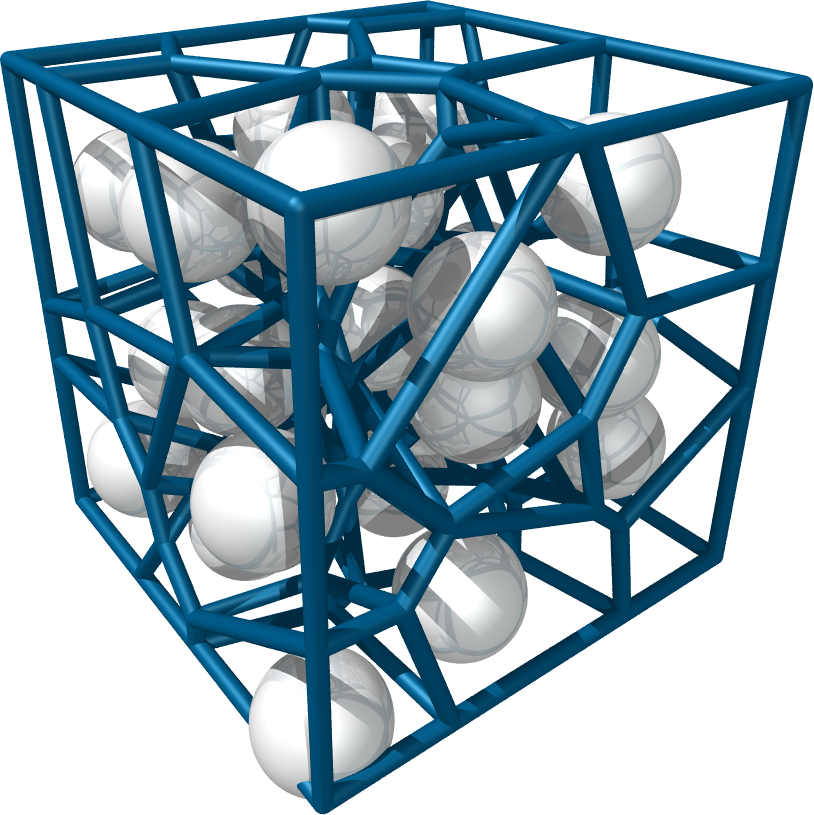
\includegraphics[height=0.7\textwidth]{images/voronoi/3d_diagram04_crop.png}%
        \caption{%
            Rendering of Voronoi cells in 3 dimensions, in a system of 27 particles. Voronoi cells created using the \cpp-library \texttt{Voro++}\cite{rycroft2009voro,webvoro++}, and rendered using the program \texttt{povray}\cite{webpovray}. %
            \label{fig:3d_voronoi_diagram}%
        }%
    \end{minipage}%
\end{figure}%

\todoa{Something about removing hydrogen atoms, and just use oxygen position as hydrogen position, and water atom ``volume''? This simplifies life for us, since we don't have to find which water molecule each hydrogen atom belongs to, but we could get inconsistent water density. But since we use the same method for all measurements, we can compare relative densities.}

\todoa{Write about averaging over timesteps and atoms}

\todob{Something about removing extreme points/tail in distribution? Caused by vacuum.}
\section{Diffusion}
\todob{derivation of diffusion? See \cite[Section~4.4.1]{frenkel2001understanding}}
When we talk about diffusion in \hl{the context of} this thesis we mean the process of \emph{self-diffusion}, which is different from \hl{``normal''} diffusion which is the net movement of a substance in the presence of a gradient, which can be for example a concentration gradient, a temperature gradient, or a pressure gradient. With \emph{self-diffusion} we mean the \hl{random?} movement in a substance that has no gradients.

Diffusion can be characterized by a constant $D$, which is related to the displacement of each atom relative to a initial position. We can measure this constant by measuring the mean square displacement $r_i^2(t)$ of each atom as a function of time, and average over all atoms. The mean square displacement is measured as
\begin{align*}
    \Braket{r^2(t)} = \frac{1}{N} \sum_{i=1}^N \left( \rvec_i(t) - \rvec_i(t=0) \right)^2,
\end{align*}
where $\rvec_i(t=0)$ is the initial position of atom $i$. From theoretical considerations of the diffusion process we can relate the diffusion constant to the mean square displacement through\cite[Section~4.4.1]{frenkel2001understanding}
\begin{align}
    \lim_{t\rightarrow \infty}\dpd{}{t}\Braket{r^2(t)} = 2dD\label{eq:diffusion_derivative}
\end{align}
where $d$ is the \hl{spatial} \hl{dimensionality/dimension?}. This means that we can find the diffusion constant in a molecular dynamics simulation by measuring the mean square displacement for many timesteps, and find the slope of this data as the diffusion constant in the limit $t\rightarrow \infty$. \hl{We are limited in that we ca not actually simulate infinite number of timesteps, but have to find a reasonable number of timesteps to measure over.} An example of how to sample the mean square displacement $\Braket{r^2(t)}$ in a simulation can be seen in \cref{list:diffusionSample}.
%
% This means that we can find the diffusion constant in a molecular dynamics simulation by measuring the mean square displacement for many timesteps, and plotting $\Braket{r^2(t)}/(2dt)$ as a function of time. The diffusion constant will then be the value this expression approaches when simulating for enough timesteps.
%
%An example of how to measure the mean square displacement in a molecular dynamics \hl{simulation/program} as outlined in \cref{chap:simple_md_program} can be seen in \cref{list:diffusionSample}.
% Fick's law relates flux $\bvec j$ of diffusing species to the concentration gradient $\bvec \nabla c$ of the species
% \begin{align*}
%     \bvec j = -D\bvec \nabla c,
% \end{align*}
% where $D$ is the proportionality constant called the diffusion \hl{coefficient/constant}.
% 
% Conservation of \hl{species/atoms?}
% \begin{align*}
%     \dpd{c(r,t)}{t} + \div \cdot \vec j(r,t) = 0,
% \end{align*}
% which gives
% \begin{align}
%     \dpd{c(r,t)}{t} - D\nabla^2 c(r,t) = 0.
%     \label{eq:diffusion_diff}
% \end{align}
% % We can solve this equation with the boundary condition
% % \begin{align*}
% %     c(r,0) = \delta (r),
% % \end{align*}
% % where $\delta(r)$ is the Dirac delta function, which gives
% % \begin{align*}
% %     c(r,t) = \frac{1}{(4\pi Dt)^{d/2}} \exp\left(-\frac{r^2}{4Dt}\right).
% % \end{align*}
% By multiplying \cref{eq:diffusion_diff} by $r^2$ and integrating over all space we get
% \begin{align*}
%     \dpd{}{t}\int \drvec~ r^2 c(r,t) = D\int \drvec~ r^2 \nabla^2 c(r,t).
% \end{align*}
% We recognize the integral on the left-hand side as the the mean square displacement %\hl{time dependence of the second moment of $c(r,t)$???}
% \todo{what???}
% \begin{align*}
%     \int \drvec~ c(r,t) r^2 \equiv \Braket{r^2(t)},
% \end{align*}
% where we have imposed
% \begin{align*}
%     \int \drvec~ c(r,t) = 1.
% \end{align*}
% Applying partial integration to the right-hand side we obtain
% \begin{align*}
%     \dpd{\Braket{r^2(t)}}{t} 
%     &= D\int \drvec~ r^2 \nabla^2 c(r,t) \\
%     &= D\int \drvec~ \div \cdot \left(r^2\nabla c(r,t)\right) - D\int\drvec~ \div r^2 \cdot \nabla c(r,t) \\
%     &= D\int \dif \vec S~ \left(r^2\div c(r,t)\right) - 2D\int\drvec~ \rvec \cdot\div c(r,t) \\
%     &= 0 - 2D\int\drvec~ (\div \cdot \rvec c(r,t)) + 2D\int\drvec~ (\div \cdot \rvec) c(r,t) \\
%     &= 0 + 2dD\int \drvec~ c(r,t) \\
%     &= 2dD
% \end{align*}
% 
% 
% \begin{align*}
%     \dpd{\Braket{r^2(t)}}{t} = 6D
% \end{align*}
% $\Rightarrow$ Plot mean square distance as function of time
% \begin{align*}
%     \Braket{\delta r(t)^2} = \frac{1}{N} \sum_{i=1}^N \delta \rvec_i(t)^2
% \end{align*}
% and find $6D$ as slope of plot \hl{(after a while?)}
%
\begin{listing}[!htb]%
\begin{cppcode*}{gobble=4}
    double diffusionSample(System &system) {
        double rSquared = 0.0;
        for (Atom *atom : system.atoms()) {
            drVec = atom->positiom() - atom->initialPosition() 
                    + atom->getBoundaryCrossings()*system.size();
            rSquared += drVec.lengthSquared();
        }
        rSquared /= system.nAtoms();
        return rSquared;
    }
\end{cppcode*}
\caption{%
    An example of how to calculate the mean square displacement in a molecular dynamics simulation. Example implementation of \mono{diffusionSample} from \cref{list:sampling}. We store the inital positions of the atoms as \mono{atom->initialPosition()}, and when using periodic boundary conditions we count the number of times we have to translate the atom one system-size in each direction, so while the position of the atom will always be inside the system, the \hl{\emph{real}} position of the atom can be calculated by adding \mono{atom->getBoundaryCrossings()*system.size()} to $\rvec$.%
    \label{list:diffusionSample}%
}%
\end{listing}%

% To improve our statistics when measuring the diffusion constant as function of distance to the surface of the pore we can use different time origins to get different samples. %
To measure $D$ we see from \cref{eq:diffusion_derivative} that we have to let $t\rightarrow \infty$, but in practice we usually see that the gradient of $\Braket{r^2(t)}$ usually have stabilzed near its final value after ${\sim} 5\text{ k}$ timesteps of 0.050 picoseconds. We can use this to get more samples for our measurements, by using different time origos. This technique involves using different initial positions for the atoms, from different timesteps in the simulation, and then finding $\Braket{r^2(t)}$ for $t_i\leq t\leq t_{i+n}$, where we $n$ is the number of timesteps we want to use for each time origo. We can in theory use overlapping intervals for $t$, but we chose to use adjacent, non-overlapping intervals. 

See \cref{fig:find_diff_const_example} for an example of how we find the diffusion constant as the gradient of $\Braket{r^2(t)}$, using different time origos.
%
% \todoao{Finish diffusion time origo stuff}
% \todoa{mention using average distance to matrix, procedure from \cref{sec:measuring_distance_to_matrix}}
% \todob{Plot of $r^2$ using standard settings ($dt$ = 20.67, 100 timesteps between states) to show approx how many origos we need to get stable gradient}
%
%
\begin{figure}[!htb]%
    \centering% 
    {
        \newcommand{\la}{\langle}%
        \newcommand{\ra}{\rangle}%
        \includesvg[width=0.8\textwidth, svgpath = ./images/diffusion/]{diffusion_constant_example02}%
    }
    \caption{%
        Illustration of how we find the diffusion constant, using two different time origos, with 40 timesteps of 0.050 picoseconds for each time origo. We find the diffusion constant as the gradient of $\langle r^2(t)\rangle/6$ for the 25 last timesteps for each origo. We then use the average of the gradients for each time origo as our approximation of $D$.%
        \label{fig:find_diff_const_example}%
    }%
\end{figure}%
% r_start = 0.0
% r_step = 0.25
% n_steps = 40
% folder_name_iterator_start = 0
% folder_name_step = 1
% folder_name_n_steps = 200
% 
% steps_per_origin = 40
%
%
% Diff const (gradient)
% 0.0295056927145
% 0.0495650040286
% 0.117231421271
% 0.0246869083899
% 0.0785722907501
% 0.156826102758


\FloatBarrier
\section{Tetrahedral order parameter}
% \todoa{Do we measure TOP for molecules or atoms?}%
% \todoa{Write about how we measure P(Q)?, since we measure probability/relative occurrence and not TOP as function of something}%
The tetrahedral order parameter\cite{errington2001relationship} is effectively a measure of how tetrahedral a set of four points are. The tetrahedral order parameter $Q$ for a point $k$ is calculated as follows%
\begin{align}
    Q_k = 1 - \frac{3}{8}\sum_i^3\sum_{j=i+1}^4 \left[ \cos \theta_{ikj} + \frac{1}{3} \right]^2,\label{eq:top_definition}
\end{align}%
%
% \begin{minipage}[c][4cm][c]{\textwidth}%
%     \begin{minipage}[c]{0.7\textwidth}%
%         \centering%
%         $Q_k = 1 - \frac{3}{8} \displaystyle\sum_i^3 \displaystyle\sum_{j=i+1}^4 \left[ \cos \theta_{ikj} + \frac{1}{3} \right]^2$%
%     \end{minipage}%
% %
%     \begin{minipage}[c]{0.25\textwidth}%
%         \centering
%         \includesvg[pretex=\normalsize, width=\textwidth, svgpath=./images/tetrahedral_order_parameter/]{tetrahedra02}%
%         \captionof{figure}{\label{hei}}
%     \end{minipage}%
%     
%     \begin{figure}[htpb]%
%         \includesvg[pretex=\normalsize, width=\textwidth, svgpath=./images/tetrahedral_order_parameter/]{tetrahedra02}%
%         \caption{a}%
%     \end{figure}%
%     
%     \caption{%
%         Illustration of the angles and molecules involved in the calculation of the tetrahedral order parameter. The \hl{blue} dots are molecules, in our case usually water molecules. We have the center molecule $k$, and \hl{its} four nearest neighbors. $\theta_{ikj}$ is the angle between molecule $i$, $k$ and $j$, as indicated by the \hl{orange} arc. \hl{FINISH CAPTION}. %
%         \label{fig:top_tetrahedra}%
%     }%
% \end{figure}%
% \end{minipage}%
% \captionof{figure}{alfa}
%
where $\theta_{ikj}$ is the angle %
%between two vectors from the main point, $k$, to point $i$ and point $j$, respectively, 
$i-k-j$ (with $k$ in the vertex of the angle) %
and the two sums go over the 6 possible angles $\theta$, between the main point and \hl{its} four nearest neighbors. See \cref{fig:top_tetrahedra} for an illustration of the angles and points involved in the calculation. If we have $Q = 1$ the four points are arranged in a perfect tetrahedron, with $\theta_{ijk} = 2\arctan(2\sqrt(2)) \approx 109.47$ for all 6 possible angles between the four points, and as the points move away from this arrangement $Q$ decreases following \cref{eq:top_definition} (negative $Q$-values are possible).
%
\begin{figure}[htpb]%
    \centering%
    \includesvg[pretex=\normalsize, width=0.3\textwidth, svgpath=./images/tetrahedral_order_parameter/]{tetrahedra02}%
    \caption{%
        Illustration of the angles and points involved in the calculation of the tetrahedral order parameter. The \hl{blue} dots are points, in our case usually water molecules. We have the center point $k$, and \hl{its} four nearest neighbors. $\theta_{ikj}$ is the angle between point $i$, $k$ and $j$, as indicated by the orange arc. \hl{FINISH CAPTION}. %
        \label{fig:top_tetrahedra}%
    }%
\end{figure}%

We use the tetrahedral order parameter for investigating the coordination of water molecules relative to other water molecules. When we lower the temperature in water below freezing the average $Q$ will \hl{approach 1/increas}, since ice has very high coordination. Liquid water also has high coordination caused by the hydrogen bonds, but much lower coordination than ice, so the distribution of $Q$-values are more spread out, with the mean lower than the mean for ice.

When we measure the tetrahedral order parameter we measure $Q$ for all water molecules, defining the position of the water molecules as the position of the oxygen atom in each molecule, and plot the \hl{relative occurrence}\todob{probability density?}, $P(Q)$, to investigate the distribution of $Q$-values. Since $Q$ isn't dependent on several timesteps (like for example diffusion), averaging over several timesteps is trivial. \todobo{But we should be wary of correlations between states?}. Since silica is hydrophilic we expect $Q$ to be different for water molecules near the silica surface, so we will measure $P(Q)$ as function of distance to the silica matrix.

% \todob{Write about time and atom average?}

% \FloatBarrier
\section{Distance to nearest atom\label{sec:distance_to_atom}}
To help visualize and characterize our nanoporous system we developed a program that creates a 3d map of the distance to the nearest atom, in each point in space on a regular grid. The implementation of this program is almost straighforward, but since we have to do a lot of calculations if we want to have a map with decent resolution, we have also parallellized the program to reduce the computation time.
\todoa{Write about distance to atom}
\todoc{Distance to atom code example?}

% \FloatBarrier
\section{Manhattan distance to nearest atom\label{sec:generation_matrix}}
Since the program from \cref{sec:distance_to_atom} takes a long time to run to get decent maps with high resolution, we decided to also develop a similar program that creates a 3d map of the space, but this time creating a map with the Manhattan distance from each point on the grid to the nearest atom. To ease calculation we this time used a method inspired by the voxelation technique from \cref{sec:voxelation}. This program first divides the system into $n_x\times n_y\times n_z$ voxels, and make a 3d matrix of the same size for storing the Manhattan distance to the nearest atom in each point. We first give all voxels with one or more atoms in them the distance 0. We then label the rest of the voxels using an iterative method, increasing the number by one for each iteration. In each iteration we find the voxels that have a neighbor voxel \hl{labelled} with the previous label (\mono{label-1}), using 4-neighbor connectivity, and give them the current label. When all voxels are labelled, they should have a label corresponding to the \hl{Manhattan distance} to the nearest atom.

Although the Manhattan distance isn't as useful as the regular Euclidean distance we calculate using the \hl{``distance to atom''}-program, the benefit is that making a 3d map of space using the \hl{``generation matrix''} method uses about 3\% of the time that ``distance to atom'' uses for the same system and same resolution. 

\todoa{Something about the usefulness of this measure?}

\orangebox{A system of 347176 atoms (\mono{rough\_fracture03}), water and SiO2, $256^3$ voxels, $~5$ seconds for ``generation matrix'', 2m27seconds for ``distance to atom'' (on one cpu)}
\todoc{Voxel counter code example?}

% \FloatBarrier
% \section{``Voxel counter''}
% \todob{Write about voxel counter}
% \todod{Voxel counter code example?}
%     A histogram of the fraction of voxels that has one or more atom in them vs. the voxel size in x-, y-, and z-direction.
%     
% % \FloatBarrier
% \section{Cage cage correlation}
%     \todod{Measure cage cage correlation}
% 
% % \FloatBarrier
% \section{Surface area of pores}
%     Only one large pore in my system, so not useful?
